% =============================================================================
% thesis-v3.tex
% 修士論文（実行条件選択モデル版）
%
% スポットインスタンス上の短時間ワークロードにおける
% 実行条件の選択による中断対策
%
% 構成:
%   第1章 序論
%   第2章 関連研究
%   第3章 中断特性の実測          <- main.tex (DPS) を基盤
%   第4章 実行条件選択のモデル     <- 新規・主役
%   第5章 実機評価の設計          <- 新規
%   第6章 結論
%
% コンパイル: lualatex thesis-v3.tex (2回)
% =============================================================================
\documentclass[11pt,a4paper]{ltjsreport}

\usepackage{luatexja}
\usepackage{amsmath,amssymb}
\usepackage{graphicx}
\usepackage{booktabs}
\usepackage{tabularx}
\usepackage{array}
\usepackage{geometry}
\usepackage{caption}
\usepackage{url}
\usepackage[hidelinks]{hyperref}

\geometry{top=30mm,bottom=30mm,left=28mm,right=28mm}
\captionsetup[figure]{labelsep=quad,font=small}
\captionsetup[table]{labelsep=quad,font=small}

\newcommand{\Fcomp}{F_{\mathrm{comp}}}
\newcommand{\Rlaunch}{R_{\mathrm{launch}}}
\newcommand{\Rint}{R_{\mathrm{int}}}
\newcommand{\Nreq}{N_{\mathrm{req}}}
\newcommand{\Nsucc}{N_{\mathrm{succ}}}
\newcommand{\Nint}{N_{\mathrm{int}}}
\newcommand{\E}{\mathbb{E}}
\newcommand{\Waste}{\mathrm{Waste}}

\title{\vspace{-10mm}
スポットインスタンス上の短時間ワークロードにおける\\
実行条件の選択による中断対策}
\author{那須 渚}
\date{2026年度 修士論文\\[2mm] 同志社大学大学院 理工学研究科}

\begin{document}
\maketitle

% =============================================================================
\chapter*{概要}
\addcontentsline{toc}{chapter}{概要}

スポットインスタンスは計算資源を低価格で利用できる一方，
提供側の都合により中断され，ジョブの再実行を要する．
CI/CD のビルドやテストのような短時間ワークロードでは，
再実行により実行時間と利用コストの双方が増加する．

本論文は，\textbf{中断によって失われる時間を最小化する実行条件を
どう選ぶか}という問いに取り組む．

まず，短時間ワークロードにおけるスポットインスタンスの信頼性を，
起動可能性ではなく\textbf{期限条件付き完了可能性} $\Fcomp(d)$，
すなわち起動に成功したインスタンスが
ワークロード期限 $d$ まで中断されずに利用可能であり続ける割合として定義し，
起動成功と起動後の中断挙動を分離して記録する
測定フレームワークを実装した．
AWS の 4 リージョン・3 インスタンスタイプを対象として
1 週間の実測（$\Nreq = 2{,}016$）を行い，
起動成功率 $96.7\%$，中断率 $6.0\%$ を観測した．
$\Fcomp(60)$ はローカル時間帯によって大きく変動し，
N.~Virginia の計算指向インスタンスでは
Night 期間の $0.98$ に対し Morning 期間で $0.69$ まで低下した．

次に，この実測値を入力として\textbf{無駄時間}，
すなわち中断による再実行で失われる時間を定式化し，
これを最小化する実行条件を選ぶ最適化問題を構築した．
無駄時間は，やり直す回数と 1 回あたりの損失の積として表され，
いずれも実測値から直接算出できる．

既存データによる評価の結果，
実行時刻を選択する戦略は，条件を選ばない場合に対して
無駄時間を\textbf{$49\%$ 削減}し（許容遅延 6 時間のとき），
完了率を $0.841$ から $0.912$ へ改善した．
効果は期限 $d$ が長いほど大きく，$d = 60$ 分で最大となる．
また期間を分割した検証により，
この効果が観測期間内の偶然によるものでないことを確認した．

さらに，リージョンおよびインスタンスタイプまで選択範囲を広げると
より大きな削減が得られるが，
これは中断が一件も観測されなかった条件を選ぶことによるものであり，
標本数の制約から確定的な結論は得られない．
この限界を明示したうえで，
実機評価の設計と必要標本数を示す．

% =============================================================================
\tableofcontents
\listoffigures
\listoftables

% =============================================================================
\chapter{序論}

\section{研究背景}

近年，クラウドコンピューティングは企業，研究機関，個人開発者によって
広く利用されている．
クラウド利用の規模が拡大し，高性能な計算資源への需要が増加するにつれて，
その利用コストは多くの利用者にとって重要な課題となっている．

コストを削減する手法の一つに，スポットインスタンスの利用がある．
スポットインスタンスは，クラウドプロバイダが余剰計算資源を
オンデマンドインスタンスより低価格で提供する料金モデルである~\cite{AWSSpot}．
オンデマンドインスタンスと比較して，
数十パーセントから最大約 90\% の割引価格で利用できる~\cite{Lin2022Survey}．
そのため，機械学習やバッチ処理のような大規模計算ワークロードだけでなく，
CI/CD における自動ビルドやテストのように
一時的に計算資源を必要とするワークロードにも利用されている~\cite{Ramesh2025}．

しかしスポットインスタンスは余剰容量に基づいて提供されるため，
クラウド需要が増加した場合や利用可能容量が減少した場合に中断されうる．
この中断を interruption event と呼ぶ．
ワークロードの実行中に interruption event が発生すると，
実行中の処理が完了前に停止する．
特にバッチ処理，機械学習，CI/CD のビルドやテストが中断された場合，
ワークロード全体の再実行が必要となり，
実行時間と利用コストの双方が増加する．

\section{問題意識}

既存のアプローチとしては，価格変動を考慮した入札戦略や，
Spot Placement Score（SPS）のようなプロバイダ固有の
可用性指標に基づく選択が挙げられる~\cite{Garg2025,Katayama2022}．
SPS は，スポットリクエストが成立する可能性を推定する上で有用である．

しかし，CI/CD パイプラインやバッチ処理ジョブのような
短時間ワークロードの利用者にとって，より実用的な問いは
\textbf{スポットインスタンスを起動できるかどうか}だけではなく，
\textbf{ワークロードが完了するまで利用し続けられるかどうか}である．

起動に成功したとしても，ワークロード完了前に中断されれば，
短時間ワークロードは失敗する．
すなわち\textbf{起動時点の可用性}と\textbf{起動後の継続性}は
異なる問題であり，既存指標は前者のみを扱っている．

\section{本研究の問い}
\label{sec:question}

本論文を貫く問いは一つである．

\begin{quote}
\textbf{中断によって失われる時間を最小化するには，
ジョブをどの条件で実行すればよいか．}
\end{quote}

この問いに答えるには，まず「失われる時間」を定量化する必要がある．

中断されるとジョブは再実行される．
したがって利用者が支払う総時間は，
本来必要な計算時間に加え，
中断された試行で費やされた時間が上乗せされる．
この上乗せ分を\textbf{無駄時間}と呼び，本論文の最小化対象とする．

無駄時間は二つの要素の積として表される．

\begin{equation}
\text{無駄時間} \;=\;
\underbrace{\text{やり直す回数}}_{\text{中断されにくさで決まる}}
\;\times\;
\underbrace{\text{1 回あたりの損失}}_{\text{中断までの経過時間で決まる}}
\label{eq:intro_waste}
\end{equation}

ここで重要なのは，\textbf{両要素がいずれも実行条件に依存する}点である．

中断されやすさは，リージョン，インスタンスタイプ，
および実行する時間帯によって異なりうる．
したがって，これらを適切に選べば無駄時間を削減できる可能性がある．

多くの CI/CD ジョブやバッチ処理は，
実行先や実行時刻を比較的柔軟に調整できる．
しかも実行条件の選択は，
\textbf{ワークロード自体の改変を必要としない}．
チェックポイント機構の実装や処理の分割といった
アプリケーション側の対応を伴わずに適用できる点で，
実務上の導入障壁が低い．

そこで本論文は，実行条件
（リージョン，インスタンスタイプ，実行時刻）を\textbf{設計変数}として扱い，
無駄時間を最小化する選択を求める問題として定式化する．

\section{本論文のアプローチ}

提案手法を設計するには，まず対象環境における
中断の実測データが必要である．
式~\eqref{eq:intro_waste} の二要素は，いずれも
「どの条件で，どの程度中断されるか」という
実測値に基づいて初めて定量化できるためである．

そこで本論文は次の順序で進める．

\begin{enumerate}
  \item \textbf{実測}（第~\ref{chap:measure} 章）：
        スポットインスタンスの信頼性を
        期限条件付き完了可能性 $\Fcomp(d)$ として定義し，
        測定フレームワークを実装して実測データを取得する．
  \item \textbf{モデル化と評価}（第~\ref{chap:model} 章）：
        実測値を入力として無駄時間を定式化し，
        これを最小化する実行条件を求める最適化問題を構築する．
        既存データにより戦略間の比較を行う．
  \item \textbf{実機評価の設計}（第~\ref{chap:plan} 章）：
        モデルの予測を実ワークロードで検証する実験を設計する．
\end{enumerate}

\section{本論文の貢献}

本論文の貢献は以下の通りである．

\begin{enumerate}
  \item 短時間ワークロードにおけるスポットインスタンスの信頼性を，
        起動可能性やインフラレベルの生存時間ではなく，
        \textbf{期限条件付き完了可能性} $\Fcomp(d)$ として定義し，
        起動成功と起動後の中断挙動を分離して記録する
        測定フレームワークを実装した（第~\ref{chap:measure} 章）．
  \item 4 リージョン・3 インスタンスタイプ・1 週間の実測により，
        $\Fcomp(d)$ がローカル時間帯によって大きく変動すること
        （$0.69$--$0.98$），および
        \textbf{中断ハザード率が経過時間によらずほぼ一定}であることを示した
        （第~\ref{chap:measure} 章）．
  \item 実測値を入力として\textbf{無駄時間を定式化}し，
        実行条件の選択を最適化問題として定式化した．
        これにより，従来は観測結果の提示にとどまっていた時間帯依存性を，
        \textbf{実行条件の決定手続き}として利用可能にした
        （第~\ref{chap:model} 章）．
  \item 既存データによる評価により，実行時刻の選択が
        無駄時間を\textbf{$49\%$ 削減}すること，
        効果が期限 $d$ に依存することを定量的に示した．
        あわせて期間分割による検証を行い，
        効果が偶然によるものでないことを確認した
        （第~\ref{chap:model} 章）．
  \item 標本数の制約により確定できない範囲を明示し，
        実機評価の設計と必要標本数を示した
        （第~\ref{chap:plan} 章）．
\end{enumerate}

\section{本論文の構成}

第~\ref{chap:related} 章では関連研究を整理する．
第~\ref{chap:measure} 章では測定フレームワークと実測結果を示す．
第~\ref{chap:model} 章では実行条件選択のモデルを構築し評価する．
第~\ref{chap:plan} 章では実機評価の設計を述べる．
第~\ref{chap:conclusion} 章で本論文をまとめる．

% =============================================================================
\chapter{関連研究}
\label{chap:related}

\section{スポットインスタンスの可用性と中断対策}

スポットインスタンスの可用性および信頼性については，
これまでに複数の研究が行われている．
Lin ら~\cite{Lin2022Survey} は可用性を向上させる手法を調査し，
チェックポイント，マイグレーション，レプリケーション，スケジューリング
といったアプローチを整理している．
これらの研究は，スポットインスタンスを実用的に利用するうえで
中断リスクが中心的課題であることを示している．

SPS は AWS が提供するプロバイダ固有の指標であり，
インスタンスタイプ，リージョン，必要容量などの条件下で
スポットリクエストが成立する可能性を推定するために用いられる~\cite{AWSSPS}．
Katayama ら~\cite{Katayama2022} はマイグレーション先の選択に SPS を用い，
起動時点の可用性を向上させられることを示した．

ただし SPS は，起動に成功したインスタンスが
ワークロードを完了するのに十分な時間
利用可能な状態を維持できるかどうかを直接示すものではない．

\section{中断挙動の時間的特性}

Kim ら~\cite{Kim2024SpotInterruption} は，
SPS が時間帯や曜日に応じて周期的に変動し，
survival time と一定の関係を持つことを示している．
Lee ら~\cite{Lee2022SpotLake} は，SPS，スポット価格，中断率などを
継続的に収集・保存するアーカイブサービス SpotLake を提案し，
GPU インスタンスや大規模インスタンスタイプで
可用性が低くなる傾向があることを報告している．

これらの研究は中断挙動の統計的性質を明らかにしているが，
時間的変動は主としてスポット市場の特性，
すなわち\textbf{観測・記述の対象}として扱われている．
観測された変動を\textbf{実行条件を決定するための入力}として
用いる枠組みは十分に検討されていない．

\section{チェックポイントによる中断対策}

中断対策としては，チェックポイントを取得して
中断時の損失を抑える手法も広く用いられている~\cite{Lin2022Survey}．
機械学習の分野ではエポック単位でのモデル保存が一般的であり，
CI/CD の分野でもテストのシャード分割といった形で
事実上の分割実行が行われている．

ただしこれらの手法は，
\textbf{ワークロード自体の改変を必要とする}．
状態の保存と復元を実装できないワークロードには適用できず，
また保存コストが大きい場合には利得が失われる．

これに対し本研究が扱う実行条件の選択は，
ワークロードに手を加えることなく適用できる．
両者は排他的ではなく併用可能であるが，
本研究は導入障壁の低い前者に焦点を当てる
（\S\ref{sec:checkpoint_discussion} で両者の関係を論じる）．

\section{本研究の位置づけ}

既存研究に対する本研究の位置づけを表~\ref{tab:related} に示す．

\begin{table}[htbp]
\centering
\caption{関連研究と本研究の位置づけ}
\label{tab:related}
\small
\begin{tabularx}{\textwidth}{@{}lXX@{}}
\toprule
 & \textbf{着目する側面} & \textbf{時間的変動の扱い} \\
\midrule
SPS~\cite{AWSSPS}，Katayama ら~\cite{Katayama2022}
  & 起動時点の可用性
  & 扱わない \\
\addlinespace
Kim ら~\cite{Kim2024SpotInterruption}，
Lee ら~\cite{Lee2022SpotLake}
  & 中断挙動の統計的性質
  & 観測・記述の対象 \\
\addlinespace
チェックポイント手法~\cite{Lin2022Survey}
  & 中断時の損失抑制
  & 扱わない（ワークロードの改変を要する） \\
\addlinespace
\textbf{本研究}
  & \textbf{期限条件付き完了可能性}
  & \textbf{実行条件を決定するための入力} \\
\bottomrule
\end{tabularx}
\end{table}

% =============================================================================
\chapter{中断特性の実測}
\label{chap:measure}

\section{本章のねらい}

第~\ref{chap:model} 章で構築するモデルは，
式~\eqref{eq:intro_waste} の二要素を定量化した値を入力として要求する．
具体的には，実行条件ごとの

\begin{itemize}
  \item 期限 $d$ まで中断されずに完了する確率
  \item 中断された場合に失われる時間の期待値
  \item インスタンスの起動オーバーヘッド
\end{itemize}

である．これらはいずれも対象環境における実測値であり，
文献値では代用できない．
本章では，これらを取得するための測定フレームワークを構築し，
AWS 上で実測を行う．

\section{期限条件付き完了可能性}

\subsection{問題の定義}

SPS のような既存指標は，スポットリクエストが成立するかどうかを特徴づける．
しかし，起動に成功したインスタンスが
ワークロード完了まで利用可能であり続けるかどうかは示さない．

CI/CD パイプラインやバッチジョブのような短時間ワークロードにとって，
この二つは異なる関心事である．
起動に成功しても完了前に中断されれば，ジョブ全体の再実行が必要となり，
実行時間とコストの双方が増加する．
したがって利用者には，リクエスト成立可能性ではなく
\textbf{期限指向のスポット信頼性}が必要である．

\subsection{指標の定義}

本研究では実際のアプリケーションレベルのワークロードは実行しない．
代わりに，指定期限まで中断されずに利用可能であることを
\textbf{ワークロード完了可能性の proxy} として用いる．
すなわち，起動に成功したインスタンスが期限 $d$ より前に
中断されなかった場合，観測条件下において
その実行時間要件を持つ短時間ワークロードは完了可能とみなす．

$\Nreq$ をスポットインスタンスの起動リクエスト数，
$\Nsucc$ を起動に成功したインスタンス数，
$\Nint(d)$ を期限 $d$ より前に中断された
起動成功インスタンス数とする．

\textbf{起動成功率}を次のように定義する．

\begin{equation}
\Rlaunch = \frac{\Nsucc}{\Nreq}
\label{eq:rlaunch}
\end{equation}

\textbf{期限前中断率}を次のように定義する．

\begin{equation}
\Rint(d) = \frac{\Nint(d)}{\Nsucc}
\label{eq:rint}
\end{equation}

さらに\textbf{期限条件付き完了可能性}を次のように定義する．

\begin{equation}
\boxed{\;\Fcomp(d) = 1 - \Rint(d)\;}
\label{eq:fcomp}
\end{equation}

この指標は，起動に成功したインスタンスのうち
期限 $d$ まで利用可能な状態を維持した割合を表す．
ただしこれは実際のアプリケーションレベルの成功率ではなく，
\textbf{インスタンスの生存に基づく proxy} として解釈すべきである．

式~\eqref{eq:rlaunch} と式~\eqref{eq:rint} を分離して定義することにより，
起動時点の容量不足に起因する失敗と，
起動後に発生する中断とを区別して分析できる．

\section{測定フレームワーク}

図~\ref{fig:framework} に測定フレームワークを示す．
本フレームワークでは，スケジューラを用いて
スポットインスタンスの起動リクエストを定期的に送信し，
起動結果，稼働状態，中断状態を収集する．

\begin{figure}[htbp]
\centering
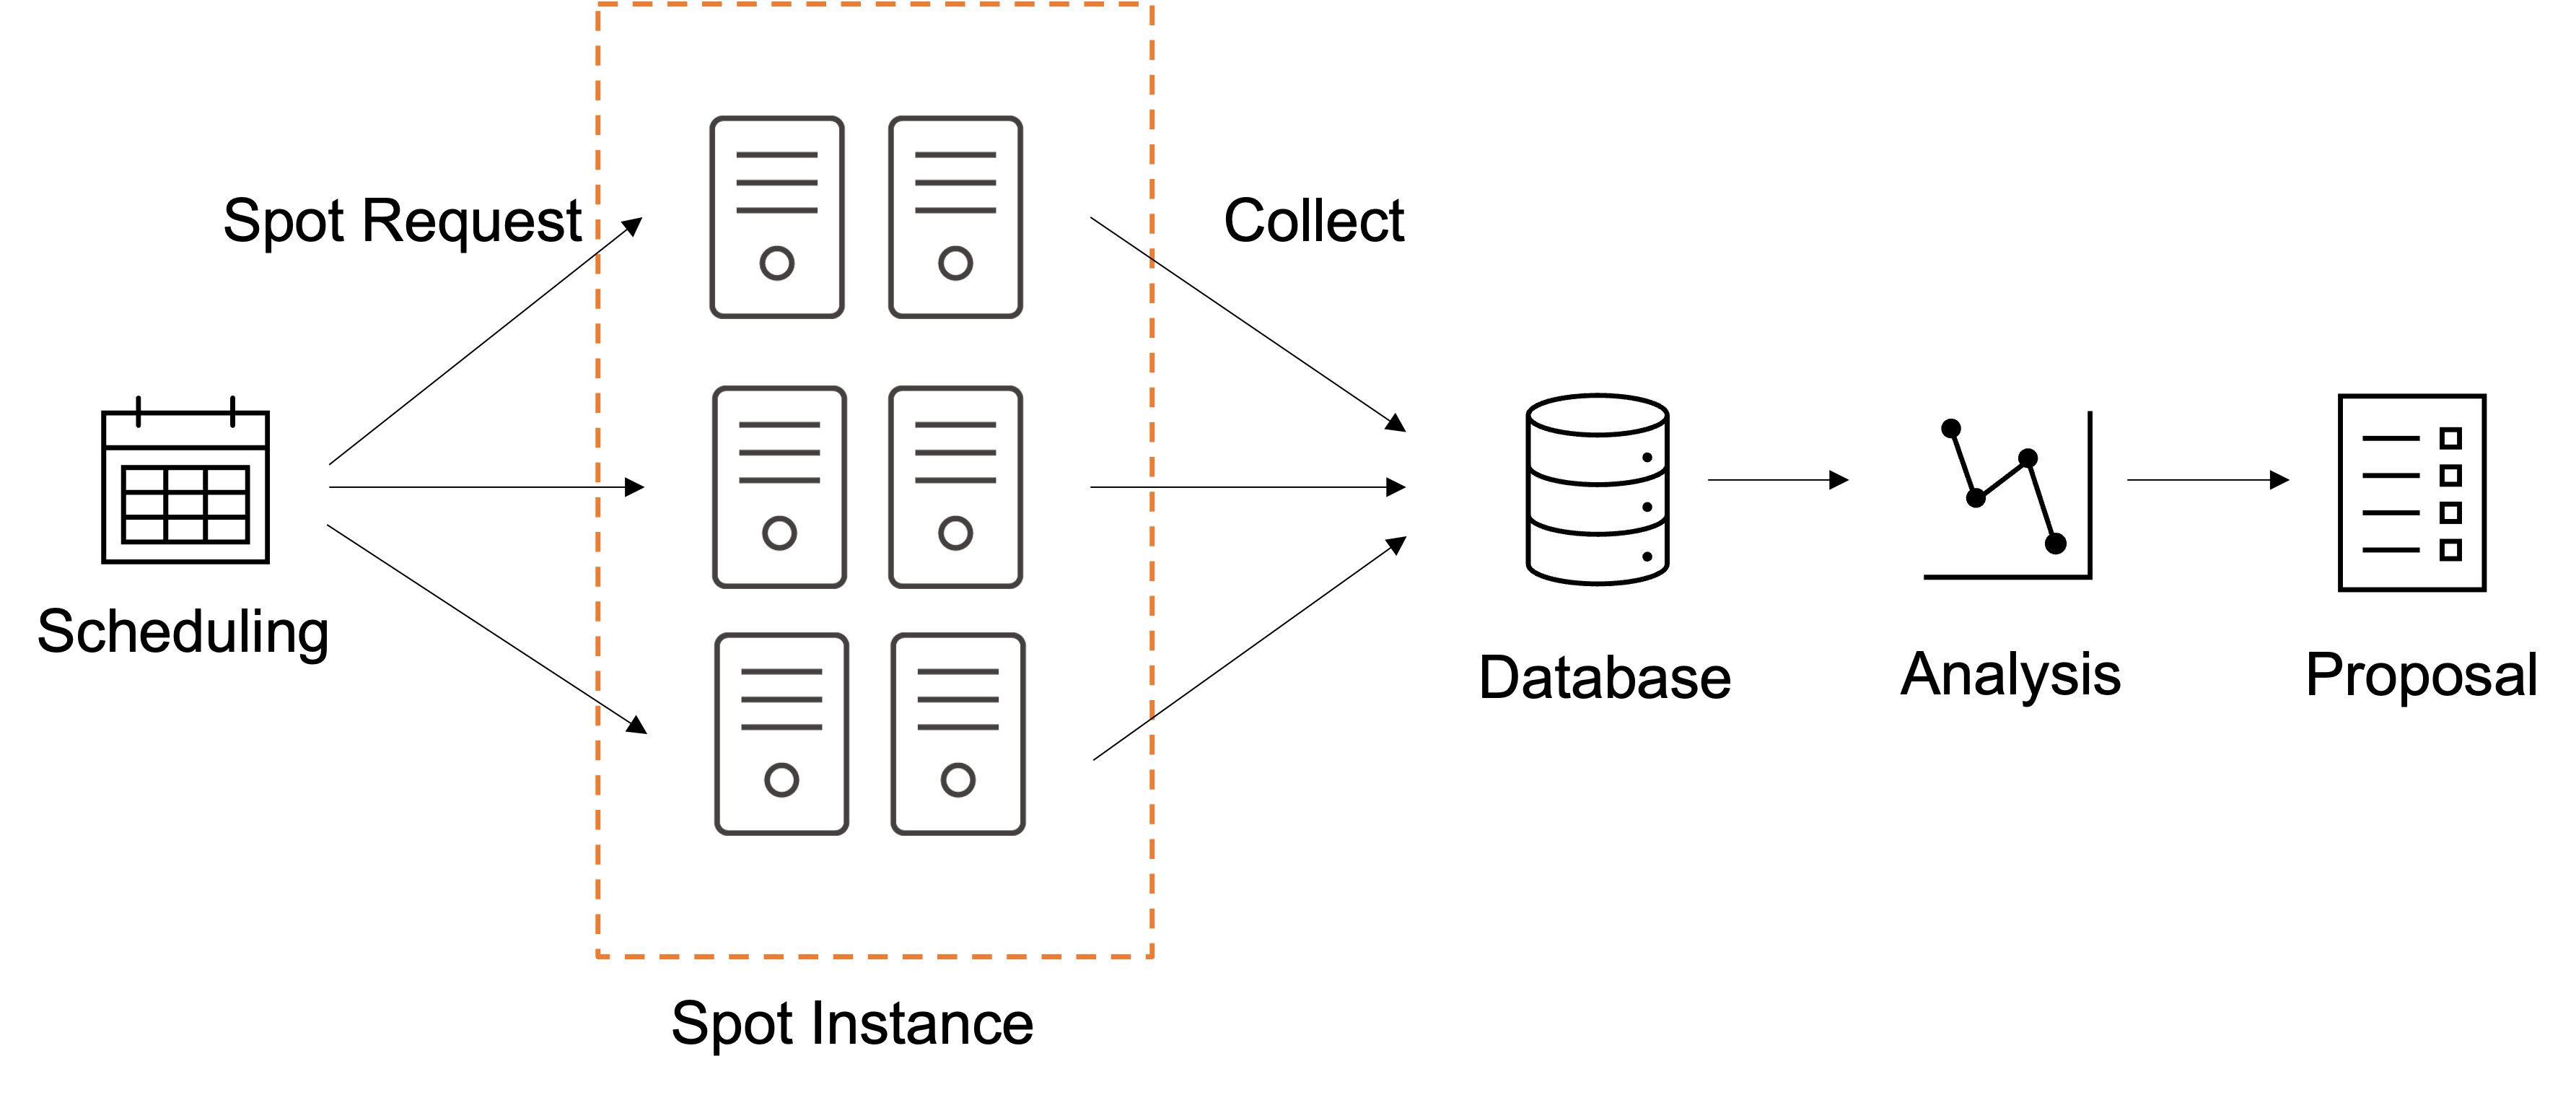
\includegraphics[width=\textwidth]{images/artect.png}
\caption{測定フレームワーク}
\label{fig:framework}
\end{figure}

スケジューラは対象とする各インスタンスタイプに対して
定期的に起動リクエストを送信する．
起動に成功した各インスタンスは 1 時間の固定観測期間にわたって監視される．
この期間中，システムはリクエストが成立したか，
インスタンスがどの程度の時間利用可能であったか，
予定終了時刻より前に interruption event が発生したかを記録する．
観測期間内に中断が発生しなかった場合，
インスタンスはシステムによって終了される．

スポット中断と通常のシステム終了を区別するため，
測定システムによって終了されることなく
予定された 1 時間の観測終了前に利用不能となったインスタンスを
中断候補として扱う．

\section{実験設定}

\paragraph{インスタンスタイプ．}
異なるリソース特性を持つインスタンスタイプ間で中断傾向を比較するため，
3 種類を代表例として選定した~\cite{Pham2018,AWSInstanceTypes}．
仕様を表~\ref{tab:specs} に示す．

\begin{table}[htbp]
\centering
\caption{評価対象インスタンスタイプの仕様。観測スポット価格は観測期間中
（2026年5月19日--25日）に 4 リージョンで記録された平均時間単価（USD/h）である。}
\label{tab:specs}
\small
\begin{tabularx}{\textwidth}{@{}l>{\raggedright\arraybackslash}X>{\raggedright\arraybackslash}X>{\raggedright\arraybackslash}X@{}}
\toprule
 & \textbf{c6a.large} & \textbf{g4dn.xlarge} & \textbf{t3.micro} \\
\midrule
分類 & 計算最適化 & GPU 搭載 & バースト可能汎用 \\
プロセッサ & AMD EPYC (3rd gen) & Intel Xeon (Cascade Lake) & Intel Xeon (burstable) \\
vCPU & 2 & 4 & 2 (burstable) \\
メモリ & 4 GiB & 16 GiB & 1 GiB \\
GPU & --- & 1$\times$ NVIDIA T4 (16 GiB) & --- \\
ローカルストレージ & EBS のみ & 125 GB NVMe SSD & EBS のみ \\
観測スポット価格 & 0.038 & 0.277 & 0.005 \\
\bottomrule
\end{tabularx}
\end{table}

\paragraph{リージョン．}
対象リージョンは N.~Virginia (us-east-1)，Tokyo (ap-northeast-1)，
Ireland (eu-west-1)，Singapore (ap-southeast-1) の 4 つである．
各リージョンにおいて，各インスタンスタイプにつき 1 時間に 1 台を起動する．

\paragraph{時間帯の区分．}
タイムスタンプを各リージョンのローカル時刻に正規化したうえで，
ローカル 1 日を 6 時間ずつの 4 区間に分割して記録する
（表~\ref{tab:periods}）．
これにより，各リージョンのローカルな需要サイクルに対して
中断傾向を比較できる．

\begin{table}[htbp]
\centering
\caption{ローカル時間帯の区分}
\label{tab:periods}
\small
\begin{tabular}{@{}ll@{}}
\toprule
区分 & ローカル時刻 \\
\midrule
Night     & 00:00--05:59 \\
Morning   & 06:00--11:59 \\
Afternoon & 12:00--17:59 \\
Evening   & 18:00--23:59 \\
\bottomrule
\end{tabular}
\end{table}

\paragraph{観測期間と価格設定．}
実験は 2026 年 5 月 19 日から 5 月 25 日まで実施した．
スポットリクエストでは最大スポット価格を指定していない．
したがって本実験は，AWS のデフォルトのスポット価格設定における
挙動を観測している．

\section{実測結果}

\subsection{全体の傾向}

観測期間中，4 リージョン・3 インスタンスタイプにわたり
合計 $\Nreq = 2{,}016$ 件の起動リクエストを送信した．
このうち $\Nsucc = 1{,}950$ 件が正常に起動し，
全体の起動成功率は $\Rlaunch = 96.7\%$ であった．
起動に成功したインスタンスのうち 117 件（$6.0\%$）が
1 時間の観測期間終了前に中断された．

期限 $d$ ごとの $\Fcomp(d)$ を表~\ref{tab:fcomp_overall} に示す．

\begin{table}[htbp]
\centering
\caption{期限 $d$ ごとの $\Fcomp(d)$（全データをプール，$\Nsucc = 1{,}950$）}
\label{tab:fcomp_overall}
\small
\begin{tabular}{@{}lrrrr@{}}
\toprule
期限 $d$ & 5 分 & 10 分 & 30 分 & 60 分 \\
\midrule
$\Fcomp(d)$ & 0.9938 & 0.9882 & 0.9692 & 0.9451 \\
\bottomrule
\end{tabular}
\end{table}

\subsection{実行条件による変動}
\label{sec:variation}

図~\ref{fig:heatmap60} に，時間帯，リージョン，
インスタンスタイプごとに集計した $\Fcomp(60)$ を示す．

\begin{figure}[htbp]
\centering
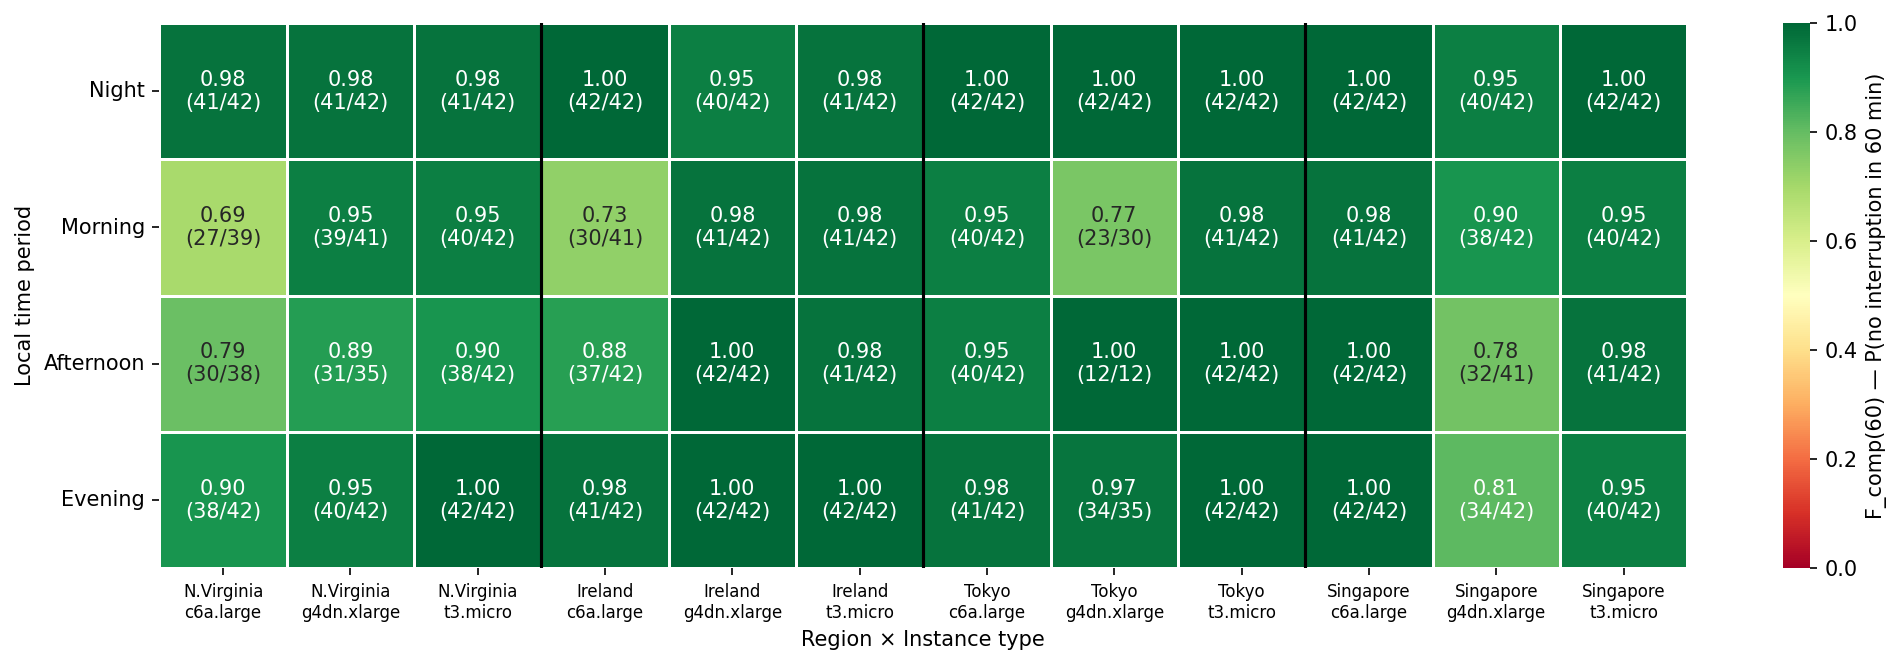
\includegraphics[width=\textwidth]{images/figure1_fcomp60_heatmap.png}
\caption{時間帯，リージョン，インスタンスタイプ別の $\Fcomp(60)$。
注釈は値とサンプル数（$n_{\mathrm{comp}}/n_{\mathrm{succ}}$）を示す。}
\label{fig:heatmap60}
\end{figure}

t3.micro はすべての条件において $\Fcomp(60) \geq 0.95$ を達成しており，
軽量インスタンスは中断に対して比較的頑健であることを示している．
一方 c6a.large および g4dn.xlarge では条件による変動が大きく，
値はおおよそ 0.65 から 1.00 の範囲で変化した．

最大の変動は N.~Virginia の c6a.large において観測された．
時間帯別の値を表~\ref{tab:period_var} に示す．

\begin{table}[htbp]
\centering
\caption{N.~Virginia，c6a.large における時間帯別の $\Fcomp(60)$}
\label{tab:period_var}
\small
\begin{tabular}{@{}lrrr@{}}
\toprule
時間帯 & $\Fcomp(60)$ & 95\% 信頼区間 & $n$ \\
\midrule
Night     & 0.98 & 0.88--1.00 & 42 \\
Morning   & 0.69 & 0.54--0.81 & 39 \\
Afternoon & 0.79 & 0.64--0.89 & 38 \\
Evening   & 0.91 & 0.78--0.96 & 42 \\
\bottomrule
\end{tabular}
\end{table}

Night と Morning の差は約 0.29 であり，
両者の信頼区間は重ならない．
この差が標本変動に起因する可能性は低い．

観測された傾向は，ローカルなクラウド需要が
日内周期に従うという仮説と整合する．
ローカル夜間には業務利用に起因する計算容量への需要が低下し，
スポットインスタンスとして利用可能な余剰容量が増加すると考えられる．
最もリスクの高い時間帯がリージョンによって異なることも
この解釈を支持する．
N.~Virginia と Ireland では Morning が最もリスクが高く，
これは北米および欧州の業務開始時間帯と対応する．
Singapore では Afternoon が最もリスクが高く，
アジア地域の午後の利用ピークと整合する．

\subsection{中断ハザード率の挙動}
\label{sec:hazard}

第~\ref{chap:model} 章のモデルは，
中断が経過時間に対してどのように発生するかに依存する．
そこで経過時間区間ごとに，その区間に入る直前まで生存していた
インスタンス数（リスク集合）で正規化したハザード率を算出した．
結果を表~\ref{tab:hazard} および図~\ref{fig:hazard} に示す．

\begin{table}[htbp]
\centering
\caption{経過時間別の中断ハザード率（$\Nsucc = 1{,}950$，中断 117 件）}
\label{tab:hazard}
\small
\begin{tabular}{@{}lrrrr@{}}
\toprule
経過時間 & 中断件数 & リスク集合 & 区間あたり & 単位時間あたり \\
\midrule
0--5 分   & 12 & 1,950 & 0.62\% & 0.123 \%/分 \\
5--10 分  & 11 & 1,938 & 0.57\% & 0.114 \%/分 \\
10--20 分 & 25 & 1,927 & 1.30\% & 0.130 \%/分 \\
20--30 分 & 12 & 1,902 & 0.63\% & 0.063 \%/分 \\
30--40 分 & 14 & 1,890 & 0.74\% & 0.074 \%/分 \\
40--50 分 & 23 & 1,876 & 1.23\% & 0.123 \%/分 \\
50--60 分 & 10 & 1,853 & 0.54\% & 0.054 \%/分 \\
\bottomrule
\end{tabular}
\end{table}

\begin{figure}[htbp]
\centering
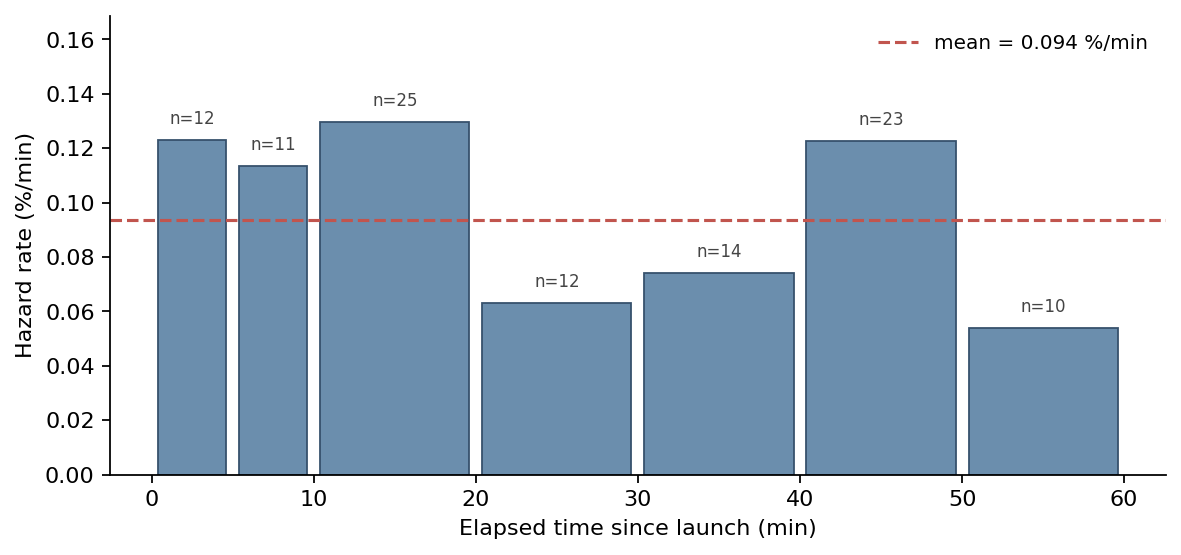
\includegraphics[width=0.85\textwidth]{images/figure3_hazard.png}
\caption{経過時間別の中断ハザード率。単調増加の傾向は見られず，
0.054--0.130 \%/分の範囲で変動する。}
\label{fig:hazard}
\end{figure}

ハザード率は 0.054--0.130 \%/分の範囲で変動するが，
\textbf{経過時間に対する単調増加の傾向は見られない}．
すなわち「長時間稼働したインスタンスほど中断されやすくなる」
という摩耗的な性質は観測されない．

この性質は第~\ref{chap:model} 章のモデルにおいて二つの含意を持つ．
第一に，中断リスクは稼働時間の経過ではなく
\textbf{実行条件によって決まる}．
したがって条件の選択が有効な対策となる．
第二に，長時間のジョブと短時間のジョブで
同一の条件選択を適用できる．

\paragraph{この主張の限界．}
中断 117 件という標本数のもとでは，
ハザードの定数性を統計的に強く主張することはできない．
本論文では「単調増加の証拠が得られなかった」という
弱い主張にとどめる．

\subsection{起動オーバーヘッド}

インスタンスの起動リクエストから実行開始までに要した時間を
表~\ref{tab:startup} に示す．

\begin{table}[htbp]
\centering
\caption{起動オーバーヘッドの実測値（$n = 1{,}950$）}
\label{tab:startup}
\small
\begin{tabular}{@{}lrrrr@{}}
\toprule
 & 平均 & 中央値 & 95 パーセンタイル & 最大 \\
\midrule
起動時間 & 4.52 秒 & 4 秒 & 6 秒 & 30 秒 \\
\bottomrule
\end{tabular}
\end{table}

\section{本章の限界}
\label{sec:limit_measure}

本章の測定にはいくつかの限界がある．

\begin{itemize}
  \item 観測期間は 1 週間に限定されており，
        各条件のサンプル数は 30--42 である．
        結果は短期的変動を反映している可能性があり，
        長期的・季節的傾向として一般化すべきではない．
  \item 中断されない状態を完了可能性の proxy としており，
        実際のアプリケーションレベルのワークロードは実行していない．
  \item 各条件につき 1 時間に 1 台のみ起動しているため，
        同時起動の影響やキュー挙動は捉えられていない．
  \item 最大スポット価格を指定していないため，
        デフォルト価格設定下の挙動のみを反映している．
\end{itemize}

\section{本章のまとめ}

本章では測定フレームワークを構築し，
AWS 上で 1 週間の実測を行った．
得られた主要な結果は以下の通りである．

\begin{enumerate}
  \item 起動成功率 $96.7\%$，中断率 $6.0\%$ を観測した．
  \item $\Fcomp(60)$ は実行条件によって $0.69$--$1.00$ の範囲で変動する．
        最大の差は N.~Virginia の c6a.large における
        Night と Morning の間の $0.29$ であり，
        信頼区間は重ならない．
  \item 中断ハザード率は経過時間によらずほぼ一定であり，
        中断リスクは稼働時間ではなく実行条件によって決まる．
  \item 起動オーバーヘッドは平均 4.52 秒である．
\end{enumerate}

結果 2 と結果 3 は，実行条件の選択が
中断対策として有効である可能性を示す．
次章ではこれを定量的なモデルとして定式化する．

% =============================================================================
\chapter{実行条件選択のモデル}
\label{chap:model}

\section{本章のねらい}

第~\ref{chap:measure} 章では，$\Fcomp(d)$ が実行条件によって
大きく変動することを示した．
しかしこの観測だけでは，
\textbf{実際にどの条件を選ぶべきか}は決まらない．

たとえば，完了可能性が最も高い条件が
最も長い待機を要する場合，それを選ぶべきかは自明でない．
また，完了可能性が同程度の条件が複数ある場合，
どちらを選んでも同じとは限らない．
中断された際に失われる時間が異なりうるからである．

本章では，実測値を入力として\textbf{無駄時間}を定式化し，
これを最小化する実行条件を求める最適化問題を構築する．
これにより，第~\ref{chap:measure} 章の観測結果を
\textbf{実行条件の決定手続き}として利用可能にする．

\section{コストモデル}
\label{sec:model_def}

\subsection{記号と決定変数}

ジョブ $j$ は時刻 $t_0$ に到着し，次で特徴づけられる．

\begin{table}[htbp]
\centering
\caption{ジョブの特徴量}
\label{tab:job}
\small
\begin{tabularx}{\textwidth}{@{}llX@{}}
\toprule
記号 & 名称 & 意味 \\
\midrule
$d$ & 実行所要時間 & ジョブの完了に要する時間（分） \\
$D$ & 許容遅延 & $t_0 + D$ までに完了すればよいという制約 \\
$\mathcal{R}$ & 利用可能リージョン & データ所在地制約などにより定まる \\
$\mathcal{T}$ & 利用可能タイプ & 必要な計算資源により定まる \\
\bottomrule
\end{tabularx}
\end{table}

決定変数は\textbf{三つ組} $(r, \tau, t)$ である．

\begin{equation}
r \in \mathcal{R}\ \text{（リージョン）},\quad
\tau \in \mathcal{T}\ \text{（インスタンスタイプ）},\quad
t\ \text{（起動時刻）}
\end{equation}

\subsection{二要素の定量化}

式~\eqref{eq:intro_waste} の二要素を，
第~\ref{chap:measure} 章の実測値を用いて書き下す．

\paragraph{第一要素：やり直す回数．}
実行条件 $(r,\tau,\pi)$ のもとで期限 $d$ まで完了する確率を
$p(r,\tau,\pi,d)$ とする．
ここで $\pi = \pi(r,t)$ は時刻 $t$ における
リージョン $r$ のローカル時間帯である．
この確率は，第~\ref{chap:measure} 章で定義・測定した
期限条件付き完了可能性そのものである．

\begin{equation}
p(r,\tau,\pi,d) \;=\; \Fcomp^{(r,\tau,\pi)}(d)
\label{eq:p_is_fcomp}
\end{equation}

成功するまで繰り返すときの試行回数は幾何分布に従い，
その期待値は $1/p$ である．
したがってやり直す回数は $1/p - 1$ となる．

\paragraph{第二要素：1 回あたりの損失．}
中断された試行で費やされた時間の期待値を

\begin{equation}
\bar u(r,\tau,\pi,d) \;=\; \E\!\left[\,U \;\middle|\; U < d\,\right]
\label{eq:ubar}
\end{equation}

とする．$U$ は観測された稼働時間であり，
第~\ref{chap:measure} 章のデータから直接算出できる．

\subsection{無駄時間}

以上より，無駄時間は次式で与えられる．

\begin{equation}
\boxed{\;
\Waste(r,\tau,t)
=
\underbrace{\left( \frac{1}{p(r,\tau,\pi(r,t),d)} - 1 \right)
            \bar u(r,\tau,\pi(r,t),d)}_{\text{やり直しによる損失}}
\;+\;
\underbrace{s}_{\text{起動}}
\;}
\label{eq:waste}
\end{equation}

ここで $s$ はインスタンス起動オーバーヘッドであり，
第~\ref{chap:measure} 章より\textbf{実測 4.52 秒}である
（表~\ref{tab:startup}）．

\textbf{本モデルの入力はすべて実測値である．}
$p$ と $\bar u$ は第~\ref{chap:measure} 章の観測データから算出され，
$s$ も同様に実測されている．
プロバイダ固有の指標や推定値を必要としない点で，
本モデルは透明かつ再現可能である．

\subsection{最適化問題}

以上より，実行条件の選択は次の最適化問題として記述される．

\begin{equation}
\begin{aligned}
\min_{r,\,\tau,\,t}\quad
  & \Waste(r,\tau,t) && \text{（無駄時間）} \\[3pt]
\text{s.t.}\quad
  & t \in [\,t_0,\; t_0 + D - d\,] && \text{（締切）} \\[2pt]
  & r \in \mathcal{R},\quad \tau \in \mathcal{T} && \text{（利用可能性）} \\[2pt]
  & p(r,\tau,\pi(r,t),d) \geq p_{\min} && \text{（信頼性下限）}
\end{aligned}
\label{eq:opt}
\end{equation}

\paragraph{許容遅延と待機可能時間．}
制約の第一式は，起動時刻 $t$ を遅らせてよい範囲を定める．
$D$ は「いつまでに完了すればよいか」，$d$ は実行所要時間であるから，
遅延させてよい上限は $D - d$ となる．
これを\textbf{slack} と呼ぶ．
slack $= 0$ のとき $t = t_0$ に退化し，
選択できるのはリージョンとタイプのみとなる．

\paragraph{信頼性下限．}
制約の第三式は，完了確率が $p_{\min}$ を下回る条件を除外する．
無駄時間の期待値が小さくとも，
完了確率が低い条件は実務上受け入れがたいためである．

\paragraph{求解．}
探索空間は，4 リージョン $\times$ 3 タイプ $\times$ 24 時刻
$= 288$ 通り程度であり，全列挙により厳密に解ける．

\section{比較する戦略}
\label{sec:strategies}

式~\eqref{eq:opt} の探索範囲を制限することにより，
以下の戦略が定義される．

\begin{table}[htbp]
\centering
\caption{比較する戦略}
\label{tab:strategies}
\small
\begin{tabularx}{\textwidth}{@{}llX@{}}
\toprule
戦略 & 探索範囲 & 位置づけ \\
\midrule
B0: Naive
  & $t = t_0$，$r,\tau$ 固定
  & 条件を選ばない。ベースライン \\
\addlinespace
B1: 時刻選択
  & $t$ を選択，$r,\tau$ 固定
  & \textbf{本章の主たる評価対象} \\
\addlinespace
B2: 条件選択
  & $r,\tau$ を選択，$t = t_0$
  & 待機を要しない \\
\addlinespace
B3: 併用
  & $r,\tau,t$ すべて選択
  & 完全版 \\
\bottomrule
\end{tabularx}
\end{table}

B1 と B2 を分離することにより，
\textbf{実行時刻の寄与}と\textbf{実行場所の寄与}を
独立に評価できる．

\section{既存データによる評価}
\label{sec:eval}

第~\ref{chap:measure} 章のデータを用いて各戦略を評価した．
到着時刻 $t_0$ は 24 時間に一様に分布すると仮定し，
各時刻について式~\eqref{eq:opt} を解いて得られる
無駄時間を平均した．
$p$ と $\bar u$ の推定には Wilson 95\% 下側信頼限界を併用し，
標本数が限られることによる楽観的推定を抑制した．

\subsection{実行時刻の選択}
\label{sec:eval_b1}

まずインスタンスタイプを c6a.large，リージョンを N.~Virginia に固定し，
実行時刻のみを選択する戦略 B1 を評価した．
結果を表~\ref{tab:b1_result} および図~\ref{fig:strategy} に示す．

\begin{table}[htbp]
\centering
\caption{実行時刻の選択による無駄時間の削減
（N.~Virginia，c6a.large，$d = 60$ 分）}
\label{tab:b1_result}
\small
\begin{tabular}{@{}lrrrr@{}}
\toprule
slack & 0 時間 & 3 時間 & 6 時間 & 12 時間 \\
\midrule
B0（条件を選ばない） & 3.94 分 & 3.94 分 & 3.94 分 & 3.94 分 \\
B1（時刻を選択）     & 3.94 分 & 2.97 分 & \textbf{2.01 分} & 1.31 分 \\
\addlinespace
削減率               & ---     & $-24\%$ & $\mathbf{-49\%}$ & $-67\%$ \\
平均完了確率 $p$     & 0.841   & 0.876   & \textbf{0.912}  & 0.958 \\
\bottomrule
\end{tabular}
\end{table}

\begin{figure}[htbp]
\centering
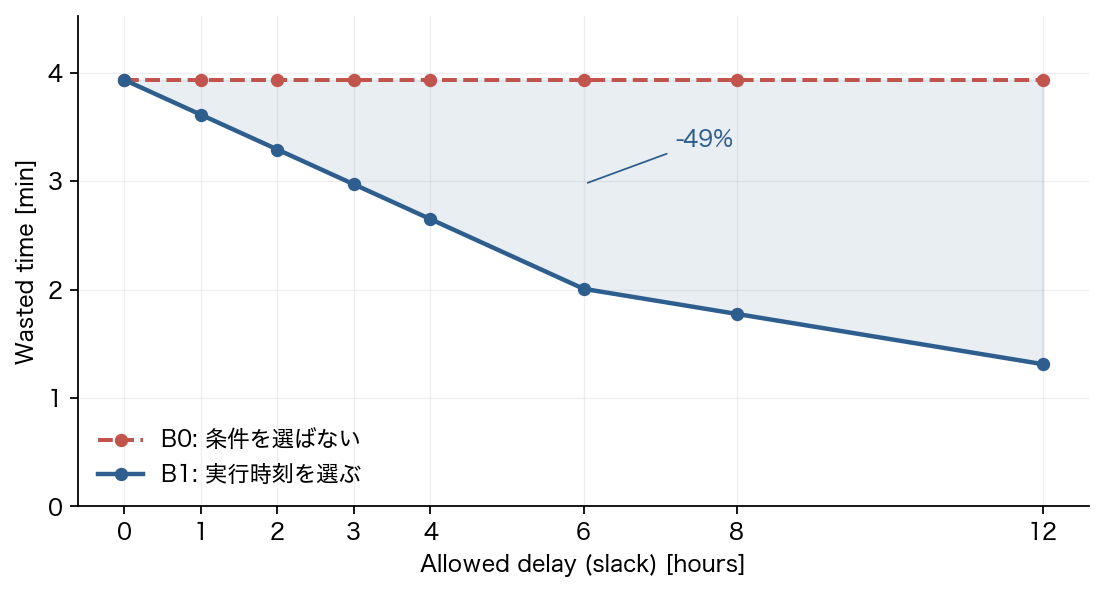
\includegraphics[width=0.85\textwidth]{images/figure6_strategy.png}
\caption{許容遅延（slack）に対する無駄時間。
slack が大きいほど選択できる時間帯が増え，無駄時間が減少する。}
\label{fig:strategy}
\end{figure}

許容遅延が 6 時間のとき，実行時刻の選択により
無駄時間は $3.94$ 分から $2.01$ 分へ\textbf{$49\%$ 削減}され，
完了確率は $0.841$ から $0.912$ へ改善した．

slack の増加に伴い削減率は単調に増加するが，
その増分は逓減する．
これは Night 期間が 6 時間しかないため，
slack が一定以上になると
最良の時間帯に到達できる到着時刻の割合が飽和するためである．

図~\ref{fig:period} に，時間帯ごとの完了可能性と無駄時間を示す．

\begin{figure}[htbp]
\centering
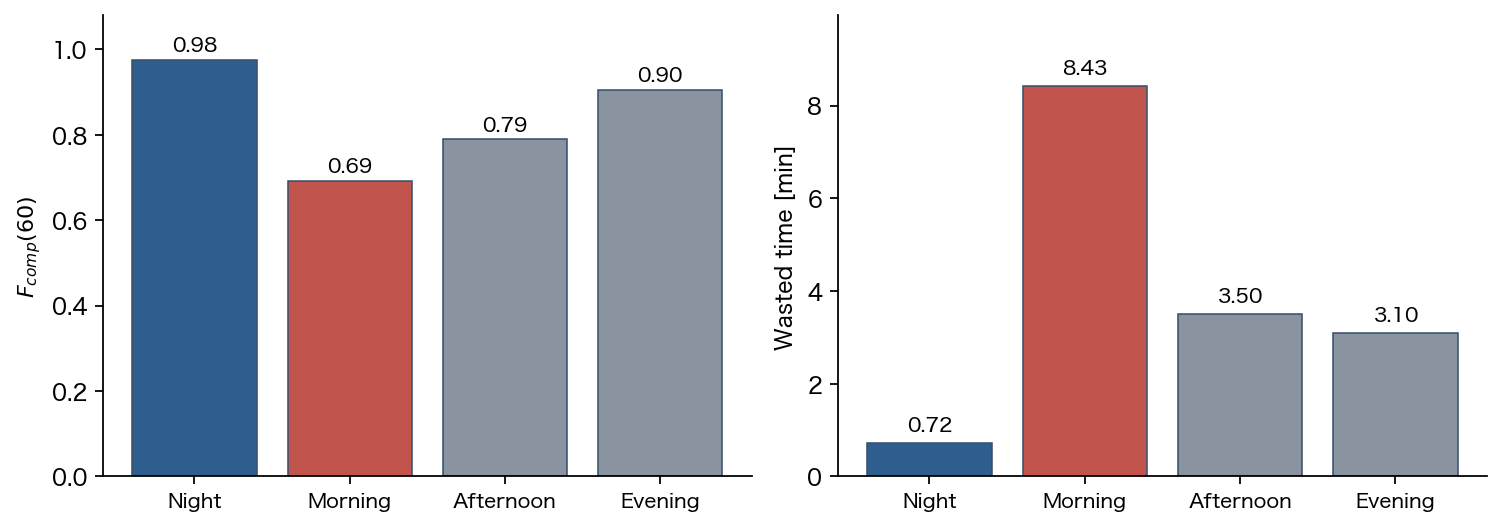
\includegraphics[width=\textwidth]{images/figure7_period.png}
\caption{N.~Virginia，c6a.large における時間帯別の
完了可能性（左）と無駄時間（右）。
Morning 期間は完了可能性が最も低く，無駄時間が最も大きい。}
\label{fig:period}
\end{figure}

\subsection{期限による効果の違い}

期限 $d$ を変化させた場合の結果を
表~\ref{tab:deadline} および図~\ref{fig:deadline} に示す．

\begin{table}[htbp]
\centering
\caption{期限 $d$ による効果の違い（slack $=$ 6 時間）}
\label{tab:deadline}
\small
\begin{tabular}{@{}lrrrr@{}}
\toprule
期限 $d$ & 5 分 & 10 分 & 30 分 & 60 分 \\
\midrule
B0 & 0.16 分 & 0.37 分 & 1.65 分 & 3.94 分 \\
B1 & 0.08 分 & 0.08 分 & 0.08 分 & 2.01 分 \\
\addlinespace
削減率 & $-53\%$ & $-80\%$ & $-95\%$ & $-49\%$ \\
\bottomrule
\end{tabular}
\end{table}

\begin{figure}[htbp]
\centering
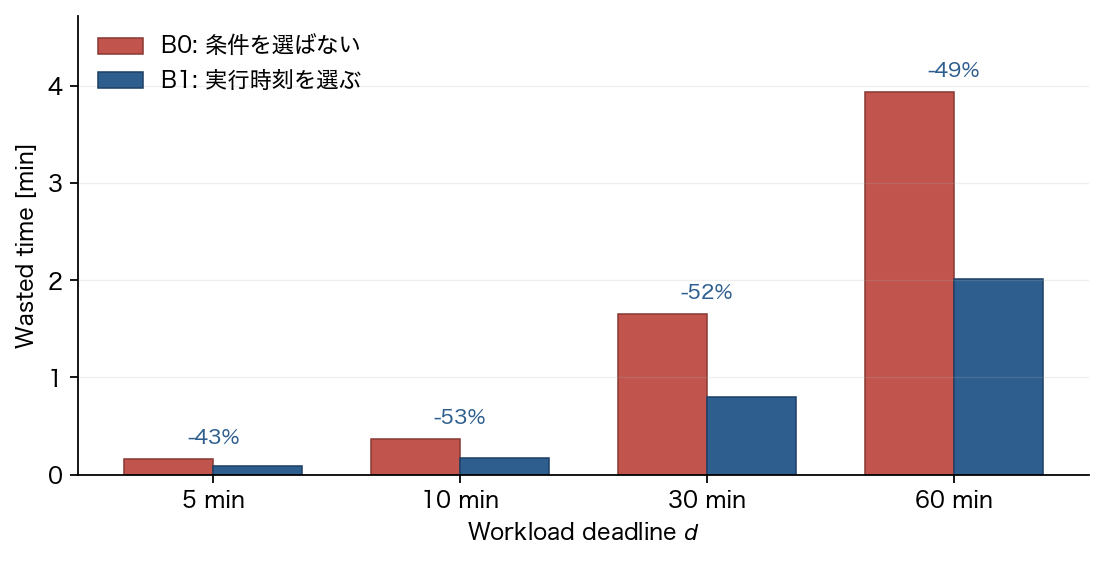
\includegraphics[width=0.85\textwidth]{images/figure8_deadline.png}
\caption{期限 $d$ による無駄時間の違い。
$d$ が長いほど無駄時間の絶対値が大きく，削減の実効的な意義も大きい。}
\label{fig:deadline}
\end{figure}

削減率は $d$ によって異なるが，
\textbf{実務上重要なのは削減率ではなく絶対値である}．
$d = 5$ 分では無駄時間が $0.16$ 分であり，
$53\%$ 削減しても $0.08$ 分の短縮にすぎない．
一方 $d = 60$ 分では $3.94$ 分から $2.01$ 分へ
$1.93$ 分の短縮となる．

したがって\textbf{実行条件の選択は，
実行時間の長いジョブにおいてより大きな意義を持つ}．

\subsection{効果の頑健性}
\label{sec:holdout}

前節の評価は，条件の選択と効果の測定に
同一のデータを用いている．
このため，観測期間内で偶然良好であった条件を選び，
その偶然を効果として計上している可能性がある．

これを検証するため，観測期間を前半 4 日と後半 3 日に分割し，
\textbf{前半のデータのみで条件を選択し，後半のデータで評価する}
手続きを行った．結果を表~\ref{tab:holdout} に示す．

\begin{table}[htbp]
\centering
\caption{期間分割による検証（$d = 60$ 分，slack $=$ 6 時間）。
前半 4 日（1,096 件）で条件を選択し，後半 3 日（854 件）で評価した。}
\label{tab:holdout}
\small
\begin{tabular}{@{}lrrr@{}}
\toprule
戦略 & 選択期間での値 & \textbf{評価期間での値} & 評価期間での削減 \\
\midrule
B0 & 8.39 分 & 1.34 分 & --- \\
B1 & 3.38 分 & \textbf{0.94 分} & $\mathbf{-30\%}$ \\
\bottomrule
\end{tabular}
\end{table}

評価期間においても B1 は B0 に対して $30\%$ の削減を示した．
選択期間での削減率（$60\%$）より小さいものの，
\textbf{効果が観測期間内の偶然のみによるものではない}ことが確認された．

なお両期間で絶対値が大きく異なるのは，
中断の発生が期間によって偏るためである．
この変動の大きさ自体が，
単一週の観測に基づく推定の不確実性を示している．

\subsection{実行場所の選択とその限界}
\label{sec:b2_limit}

リージョンおよびインスタンスタイプまで選択範囲を広げた場合
（戦略 B2，B3）の結果を表~\ref{tab:b2_result} に示す．

\begin{table}[htbp]
\centering
\caption{選択範囲を広げた場合の無駄時間（$d = 60$ 分，slack $=$ 6 時間）}
\label{tab:b2_result}
\small
\begin{tabular}{@{}llrr@{}}
\toprule
戦略 & 選択範囲 & 無駄時間 & 削減率 \\
\midrule
B0 & なし & 3.94 分 & --- \\
B1 & 時刻 & 2.01 分 & $-49\%$ \\
B2 & 場所（リージョン・タイプ） & 0.10 分 & $-97\%$ \\
B3 & 時刻 $+$ 場所 & 0.08 分 & $-98\%$ \\
\bottomrule
\end{tabular}
\end{table}

B2 および B3 は B1 を大きく上回る削減を示している．
しかし\textbf{この値はそのまま受け取るべきではない}．

B2 と B3 が選択するのは Tokyo の Night 期間であるが，
この条件では観測期間中に\textbf{中断が一件も発生していない}
（$n = 42$，中断 0 件）．
このため完了確率の推定値は $1.00$ となり，
式~\eqref{eq:waste} の無駄時間はほぼ $0$ に評価される．

問題は，48 条件のうち\textbf{15 条件（$31\%$）で
中断が一件も観測されていない}ことである．
中断 117 件が 48 条件に分散するため，
$n \approx 40$ の標本では偶然 0 件となる条件が多数生じる．
したがって完了確率 $1.00$ は
「中断しない」ことを意味せず，
「観測されなかった」ことを意味するにすぎない．

\paragraph{本論文の立場．}
以上より，本論文では\textbf{B1（実行時刻の選択）を主たる結果とする}．
B1 は同一リージョン内の時間帯比較であり，
比較するすべての時間帯で中断が実際に観測されている
（表~\ref{tab:period_var}）．
したがって推定値は観測に裏付けられている．

一方 B2 および B3 については，
\textbf{さらなる削減の余地があることを示唆するにとどめ，
確定的な結論は述べない}．
これらの確認には標本数の増加が必要であり，
第~\ref{chap:plan} 章の実機評価の対象とする．

\section{考察}

\subsection{なぜ実行条件の選択が有効か}

第~\ref{chap:measure} 章で観測されたハザード率の挙動
（\S\ref{sec:hazard}）が，本章の結果を説明する．

中断ハザード率が経過時間によらずほぼ一定であることは，
中断リスクが\textbf{稼働時間の長さではなく実行条件によって決まる}
ことを意味する．
長時間稼働したインスタンスが摩耗的に中断されやすくなるのであれば，
条件を選んでも時間の経過とともにリスクが蓄積し，
効果は限定的となる．
しかし実測ではそのような傾向は見られなかった．

したがって，中断されにくい条件を選べば，
その低いリスクが実行期間を通じて維持される．
これが実行条件の選択が有効である理由である．

\subsection{チェックポイントによる対策との関係}
\label{sec:checkpoint_discussion}

中断対策としては，ジョブを分割してチェックポイントを取得し，
中断時の損失を抑える手法も広く用いられている．
本研究の枠組みにおいて，この手法は
式~\eqref{eq:intro_waste} の第二要素
（1 回あたりの損失）を削減するものと位置づけられる．

両者は排他的ではなく，併用可能である．
しかしチェックポイントによる対策には
\textbf{ワークロード自体の改変が必要}であり，
状態の保存と復元を実装できないワークロードには適用できない．

また予備的な分析によれば，
チェックポイントの保存および復元に要する時間が
60 秒を超える場合，分割による利得は失われる．
中断率が $6.0\%$ と低いため，
中断が発生しない大部分の実行において
保存コストが無駄となるためである．

これに対し実行条件の選択は，
ワークロードに手を加えることなく適用でき，
保存コストを伴わない．
本研究がこの手法に焦点を当てる理由である．

\subsection{実務上の含意}

本章のモデルは，実務者に対して次の手続きを与える．

\begin{enumerate}
  \item 対象環境において $\Fcomp(d)$ と $\bar u$ を測定する
        （第~\ref{chap:measure} 章の枠組みによる）．
  \item ジョブの許容遅延 $D$ と所要時間 $d$ から slack を求める．
  \item 式~\eqref{eq:opt} を解き，実行条件を決定する．
\end{enumerate}

この手続きはプロバイダ固有の指標を必要とせず，
自身の観測データのみに基づく．
また第~\ref{chap:measure} 章で示したとおり，
最もリスクの高い時間帯はリージョンによって異なるため，
\textbf{単一の普遍的な規則を適用するのではなく，
対象環境での測定に基づいて決定すべきである}．

\section{本章のまとめ}

本章では，実測値を入力として無駄時間を定式化し，
実行条件の選択を最適化問題として構築した．

得られた主要な結果は以下の通りである．

\begin{enumerate}
  \item 無駄時間は式~\eqref{eq:waste} として定式化され，
        その入力はすべて第~\ref{chap:measure} 章の実測値から得られる．
  \item 実行時刻の選択により，無駄時間は $49\%$ 削減され
        （slack $=$ 6 時間），完了確率は $0.841$ から $0.912$ へ改善する．
  \item 効果は期限 $d$ が長いほど絶対値として大きく，
        $d = 60$ 分で $1.93$ 分の短縮となる．
  \item 期間分割による検証により，
        評価期間においても $30\%$ の削減が確認された．
  \item 実行場所まで選択範囲を広げるとさらなる削減が示唆されるが，
        中断が観測されなかった条件に依存するため，
        確定的な結論は得られない．
\end{enumerate}

結果 5 が示すとおり，本章の評価は
単一週の観測データに基づく限界を持つ．
次章では，これを実ワークロードで検証する実験を設計する．

% =============================================================================
\chapter{実機評価の設計}
\label{chap:plan}

\section{検証すべき事項}

第~\ref{chap:model} 章の評価は，
第~\ref{chap:measure} 章で取得した観測データに基づく
シミュレーションである．
実際のワークロードを実行したものではない．

そこで本章では，モデルの予測を実機で検証する実験を設計する．
検証すべき事項を優先順位とともに表~\ref{tab:objectives} に示す．

\begin{table}[htbp]
\centering
\caption{検証の目的と優先順位}
\label{tab:objectives}
\small
\begin{tabularx}{\textwidth}{@{}clX@{}}
\toprule
優先 & 目的 & 理由 \\
\midrule
1 & \textbf{B1 の効果の実証}
  & 本論文の主たる主張。予測値（無駄時間 $-49\%$，
    完了確率 $+7$ ポイント）が実ワークロードで再現されるか \\
\addlinespace
2 & モデルの予測精度
  & 式~\eqref{eq:waste} による予測値と実測値の乖離 \\
\addlinespace
3 & B2・B3 の確認
  & \S\ref{sec:b2_limit} で確定できなかった，
    実行場所の選択による追加的な削減 \\
\addlinespace
4 & 中断の独立性
  & 期待試行回数 $1/p$ の前提の検証 \\
\bottomrule
\end{tabularx}
\end{table}

\section{実験 1：実行時刻選択の効果の実証}

\paragraph{目的．}
戦略 B1 の効果を実ワークロードで検証する．

\paragraph{設計．}
対照群と処理群を並行して実行する．

\begin{table}[htbp]
\centering
\caption{実験 1 の設計}
\label{tab:exp1}
\small
\begin{tabularx}{\textwidth}{@{}lX@{}}
\toprule
項目 & 内容 \\
\midrule
対照群（B0） & 到着時刻にそのまま実行 \\
処理群（B1） & 式~\eqref{eq:opt} の解に従い，許容遅延 6 時間以内で
               無駄時間が最小となる時刻に実行 \\
\addlinespace
リージョン & N.~Virginia（固定） \\
インスタンスタイプ & c6a.large（固定） \\
ワークロード & 60 分の実ジョブ。チェックポイント機構を持たないもの \\
到着時刻 & 毎時 0 分（1 日 24 回） \\
\bottomrule
\end{tabularx}
\end{table}

リージョンとタイプを固定するのは，
\S\ref{sec:b2_limit} で述べたとおり，
実行場所の選択が標本数の制約を受けるためである．
本実験では\textbf{実行時刻の効果のみを分離して検証する}．

\paragraph{測定項目．}

\begin{itemize}
  \item 完了率：期限 60 分までに中断されなかった割合
  \item やり直し回数
  \item 無駄時間：中断された試行で費やされた時間の合計
  \item 完了までの実時間
\end{itemize}

\paragraph{予測値．}
第~\ref{chap:model} 章のモデルによる予測を
表~\ref{tab:prediction} に示す．

\begin{table}[htbp]
\centering
\caption{実験 1 で検証すべき予測値（$d = 60$ 分，slack $=$ 6 時間）}
\label{tab:prediction}
\small
\begin{tabular}{@{}lrrr@{}}
\toprule
指標 & B0 & B1 & 差 \\
\midrule
完了確率 & 0.841 & 0.912 & $+7.1$ ポイント \\
無駄時間 & 3.94 分 & 2.01 分 & $-49\%$ \\
やり直し率 & 15.9\% & 8.8\% & $-7.1$ ポイント \\
\bottomrule
\end{tabular}
\end{table}

\paragraph{必要標本数．}
完了確率の差（$7.1$ ポイント）を
有意水準 $5\%$，検出力 $80\%$ で検出するために必要な標本数は，
両群合計で約 $690$ 件である\footnote{%
二標本比率の検定における標本サイズの近似式
$n \approx 16\,\bar p(1-\bar p)/\delta^{2}$（片群あたり）による。
$\bar p = 0.877$，$\delta = 0.071$ として片群約 $344$ 件，
両群計約 $687$ 件。正確な式によれば両群計約 $671$ 件であり，
以下では安全側をとって $690$ 件とする。}．
1 日 24 回・両群で 48 件を実行する場合，
\textbf{約 15 日}で必要な標本数に達する．

\paragraph{コスト．}
c6a.large の観測スポット価格（$0.0295$ USD/h）に基づくと，
$690$ 件 $\times$ 1 時間 $\times$ $0.0295$ USD
$\approx$ \textbf{\$20} である．

\section{実験 2：実行場所の選択}

\paragraph{目的．}
\S\ref{sec:b2_limit} で確定できなかった
B2・B3 の効果を検証する．

\paragraph{設計．}
実験 1 と並行し，4 リージョンで同一のワークロードを実行する．
とりわけ，中断が観測されなかった条件
（Tokyo の Night 期間など）について標本を追加する．

\paragraph{規模．}
各条件の標本数を 100 件以上とするには，
4 リージョン $\times$ 4 時間帯 $\times$ 100 件
$= 1{,}600$ 件の実行を要する．
1 日 96 件（4 リージョン $\times$ 24 回）で約 17 日である．
コストは約 \$47 である．

\section{実験 3：中断の独立性の検証}

\paragraph{目的．}
「中断された直後の再試行も同じ確率 $p$ で成功する」
という仮定を検証する．

式~\eqref{eq:waste} における期待試行回数 $1/p$ は，
各試行が独立であることを前提としている．
しかし中断は容量逼迫時に発生すると考えられるため，
直後の再試行はより失敗しやすい可能性がある．
その場合 $p$ は過大評価であり，
本論文の削減率も割り引いて解釈する必要がある．

\paragraph{方法．}
中断を検知した場合に即座に同一条件で再起動し，
2 回目の成否を記録する．
1 回目の $p$ と 2 回目の $p$ を比較する．

\paragraph{規模．}
\textbf{実験 1 および 2 に相乗りできる}．
中断された実行について再試行の結果を記録すればよく，
追加のコストを要しない．
中断率 $6.0\%$ のもとでは，
実験 1 と 2 を合わせた約 $2{,}290$ 件から
約 $137$ 件の中断が得られる見込みである．

\section{実験規模のまとめ}

\begin{table}[htbp]
\centering
\caption{実験の規模とコスト}
\label{tab:exp_scale}
\small
\begin{tabularx}{\textwidth}{@{}llrX@{}}
\toprule
実験 & 期間 & コスト & 得られるもの \\
\midrule
1: B1 の実証 & 約 15 日 & \$20 & \textbf{本論文の主張の検証} \\
2: B2・B3 の確認 & 約 17 日 & \$47 & 実行場所の選択の効果 \\
3: 独立性 & 実験 1・2 に相乗り & \$0 & モデルの前提の検証 \\
\midrule
\textbf{合計} & \textbf{約 3 週間} & \textbf{約 \$67} & \\
\bottomrule
\end{tabularx}
\end{table}

実験 1 と 2 は並行実行できるため，
全体で約 3 週間を見込む．

\section{実装方針}

第~\ref{chap:measure} 章で構築した測定フレームワークを流用する．
変更点を表~\ref{tab:impl} に示す．

\begin{table}[htbp]
\centering
\caption{既存実装からの変更点}
\label{tab:impl}
\small
\begin{tabularx}{\textwidth}{@{}lX@{}}
\toprule
既存要素 & 変更内容 \\
\midrule
起動処理 & 待機処理を実ワークロードに置換 \\
中断検知 & そのまま流用（インスタンスメタデータの監視） \\
スケジューラ & 戦略に従って起動時刻を決定する処理を追加。
               待機中は起動予約のみを登録し，計算資源を占有しない \\
記録項目 & 戦略名，到着時刻，実際の起動時刻，再試行回数を追加 \\
\bottomrule
\end{tabularx}
\end{table}

\section{想定される結果}

実験 1 の結果に応じて，導かれる結論を
表~\ref{tab:outcomes} に示す．
\textbf{いずれの場合も報告価値のある結果となる}．

\begin{table}[htbp]
\centering
\caption{実験 1 の結果に応じた結論}
\label{tab:outcomes}
\small
\begin{tabularx}{\textwidth}{@{}lX@{}}
\toprule
実測結果 & 導かれる結論 \\
\midrule
予測と整合
  & 実行条件の選択が有効であり，
    式~\eqref{eq:waste} が実環境を説明できることが示される \\
\addlinespace
効果はあるが予測より小さい
  & 効果の存在は確認されるが，モデルの前提
    （とりわけ試行の独立性）に修正が必要である \\
\addlinespace
効果が認められない
  & 観測期間と実験期間の間でスポット市場が変化したか，
    単一週の観測に基づく推定が一般化できないことを示す。
    \textbf{観測の有効期間という新たな問いが生じる} \\
\bottomrule
\end{tabularx}
\end{table}

\section{リスクと対策}

\begin{table}[htbp]
\centering
\caption{想定されるリスクと対策}
\label{tab:risks}
\small
\begin{tabularx}{\textwidth}{@{}XXX@{}}
\toprule
リスク & 影響 & 対策 \\
\midrule
中断が十分に集まらない
  & 検出力の不足
  & 中断率が最も高い条件（N.~Virginia，Morning）を
    対照群の実行対象に含める \\
\addlinespace
観測期間と実験期間の市場変化
  & 予測が外れる
  & 実験期間中に $\Fcomp$ を再測定し，
    第~\ref{chap:measure} 章の値と比較する \\
\addlinespace
独立性が成立しない
  & $p$ が過大評価となる
  & 実験 3 で検証し，必要なら条件付き確率へ修正する \\
\addlinespace
実ワークロードの失敗が混入
  & 中断と区別できない
  & ジョブの終了コードと中断通知を分けて記録する \\
\bottomrule
\end{tabularx}
\end{table}

% =============================================================================
\chapter{結論}
\label{chap:conclusion}

\section{本論文のまとめ}

本論文は，\textbf{中断によって失われる時間を最小化するには
ジョブをどの条件で実行すればよいか}という問いに取り組んだ．

第~\ref{chap:measure} 章では，スポットインスタンスの信頼性を
期限条件付き完了可能性 $\Fcomp(d)$ として定義し，
起動成功と起動後の中断挙動を分離して記録する
測定フレームワークを実装した．
AWS の 4 リージョン・3 インスタンスタイプを対象として
1 週間の実測（$\Nreq = 2{,}016$）を行い，
起動成功率 $96.7\%$，中断率 $6.0\%$ を観測した．
$\Fcomp(60)$ は実行条件によって $0.69$--$1.00$ の範囲で変動し，
最大の差は N.~Virginia の c6a.large における
Night 期間と Morning 期間の間の $0.29$ であった．
また中断ハザード率は経過時間によらずほぼ一定であり，
中断リスクが稼働時間ではなく実行条件によって決まることを示した．

第~\ref{chap:model} 章では，これらの実測値を入力として
\textbf{無駄時間}を定式化し，
実行条件の選択を最適化問題として構築した．
本モデルの入力はすべて実測値であり，
プロバイダ固有の指標を必要としない．
既存データによる評価の結果，
実行時刻の選択により無駄時間は\textbf{$49\%$ 削減}され
（許容遅延 6 時間のとき），
完了確率は $0.841$ から $0.912$ へ改善した．
また期間を分割した検証により，
評価期間においても $30\%$ の削減が確認され，
効果が観測期間内の偶然のみによるものでないことを示した．

一方，実行場所まで選択範囲を広げた場合には
より大きな削減が示唆されたが，
これは中断が一件も観測されなかった条件に依存するものであり，
標本数の制約から確定的な結論は得られなかった．
この限界を明示したうえで，
第~\ref{chap:plan} 章では実機評価の設計と
必要標本数（両群計約 $690$ 件，約 3 週間，約 \$67）を示した．

\section{本研究の意義}

本研究の意義は以下の三点である．

\begin{enumerate}
  \item スポットインスタンスの信頼性を，
        プロバイダ固有の不透明な指標ではなく，
        直接観測された起動・中断記録のみから算出される
        \textbf{解釈可能な指標}として定式化した．
  \item 従来は観測・記述の対象として扱われてきた中断挙動の時間的変動を，
        \textbf{実行条件を決定するための入力}として利用する
        枠組みを与えた．
        これにより，観測結果が実行条件の決定手続きとして
        利用可能になる．
  \item 提案手法は\textbf{ワークロード自体の改変を必要としない}．
        チェックポイント機構の実装や処理の分割を伴わずに
        適用できる点で，実務上の導入障壁が低い．
\end{enumerate}

\section{今後の課題}

\begin{itemize}
  \item 第~\ref{chap:plan} 章の実機評価の実施
  \item 観測期間の延長による，季節変動を含む長期的傾向の把握，
        および観測結果の有効期間の検討
  \item 実行場所の選択（B2・B3）の効果の確定
  \item 中断の独立性に関する検証と，
        成立しない場合のモデルの修正
  \item チェックポイントによる対策との併用効果の検討
  \item SPS など既存のプロバイダ固有指標との定量的比較
\end{itemize}

% =============================================================================
\chapter*{謝辞}
\addcontentsline{toc}{chapter}{謝辞}

本研究を進めるにあたり，終始丁寧なご指導を賜りました
指導教員の先生方に深く感謝いたします．
また，日頃より有益な議論をいただいた研究室の皆様に御礼申し上げます．

% =============================================================================
\begin{thebibliography}{99}
\addcontentsline{toc}{chapter}{参考文献}

\bibitem{AWSSpot}
Amazon Web Services:
Amazon EC2 Spot Instances.
\url{https://aws.amazon.com/ec2/spot/}
(Accessed: May 2026)

\bibitem{Lin2022Survey}
Lin, L., Pan, L., Liu, S.:
Methods for improving the availability of spot instances: A survey.
Computers in Industry, 141, 103718 (2022).

\bibitem{Ramesh2025}
Ramesh, D.G.A., Lennon, R.G.:
Evaluating the Impact of Reserved Instances vs. Spot Instances in DevOps Cloud Workflows.
In: 2025 35th Irish Signals and Systems Conference (ISSC). IEEE (2025).

\bibitem{Garg2025}
Garg, D., Kaata, S.K., Bhumireddy, D.R., Bolla, B.K.:
Reducing Cloud Cost Through Optimized Bidding for AWS Spot Instances.
In: 2025 3rd International Conference on Advances in Computation,
Communication and Information Technology (ICAICCIT). IEEE (2025).

\bibitem{Katayama2022}
Katayama, D., Kasai, K., Koita, T.:
Migration Destination Selection Algorithm for Spot Instances using SPS.
In: 2022 IEEE International Conference on Big Data (Big Data),
pp. 6690--6692. IEEE, Osaka (2022).

\bibitem{Kim2024SpotInterruption}
Kim, K., Lee, K.:
Making Cloud Spot Instance Interruption Events Visible.
In: Proceedings of the ACM Web Conference 2024 (WWW '24),
pp. 2998--3009. ACM, New York (2024).

\bibitem{AWSSPS}
Amazon Web Services:
Spot Placement Score. Amazon EC2 User Guide.
\url{https://docs.aws.amazon.com/AWSEC2/latest/UserGuide/spot-placement-score.html}
(Accessed: May 2026)

\bibitem{Lee2022SpotLake}
Lee, S., Hwang, J., Lee, K.:
SpotLake: Diverse Spot Instance Dataset Archive Service.
In: 2022 IEEE International Symposium on Workload Characterization (IISWC),
pp. 242--255. IEEE (2022).

\bibitem{Pham2018}
Pham, T.-P., Ristov, S., Fahringer, T.:
Performance and Behavior Characterization of Amazon EC2 Spot Instances.
In: 2018 IEEE 11th International Conference on Cloud Computing (CLOUD).
IEEE (2018).

\bibitem{AWSInstanceTypes}
Amazon Web Services:
Amazon EC2 Instance Types. Amazon EC2 User Guide.
\url{https://docs.aws.amazon.com/AWSEC2/latest/UserGuide/instance-types.html}
(Accessed: May 2026)

\end{thebibliography}

\end{document}
